\begin{figure}[t]
	\centering
    \subfloat[Load Time]
    {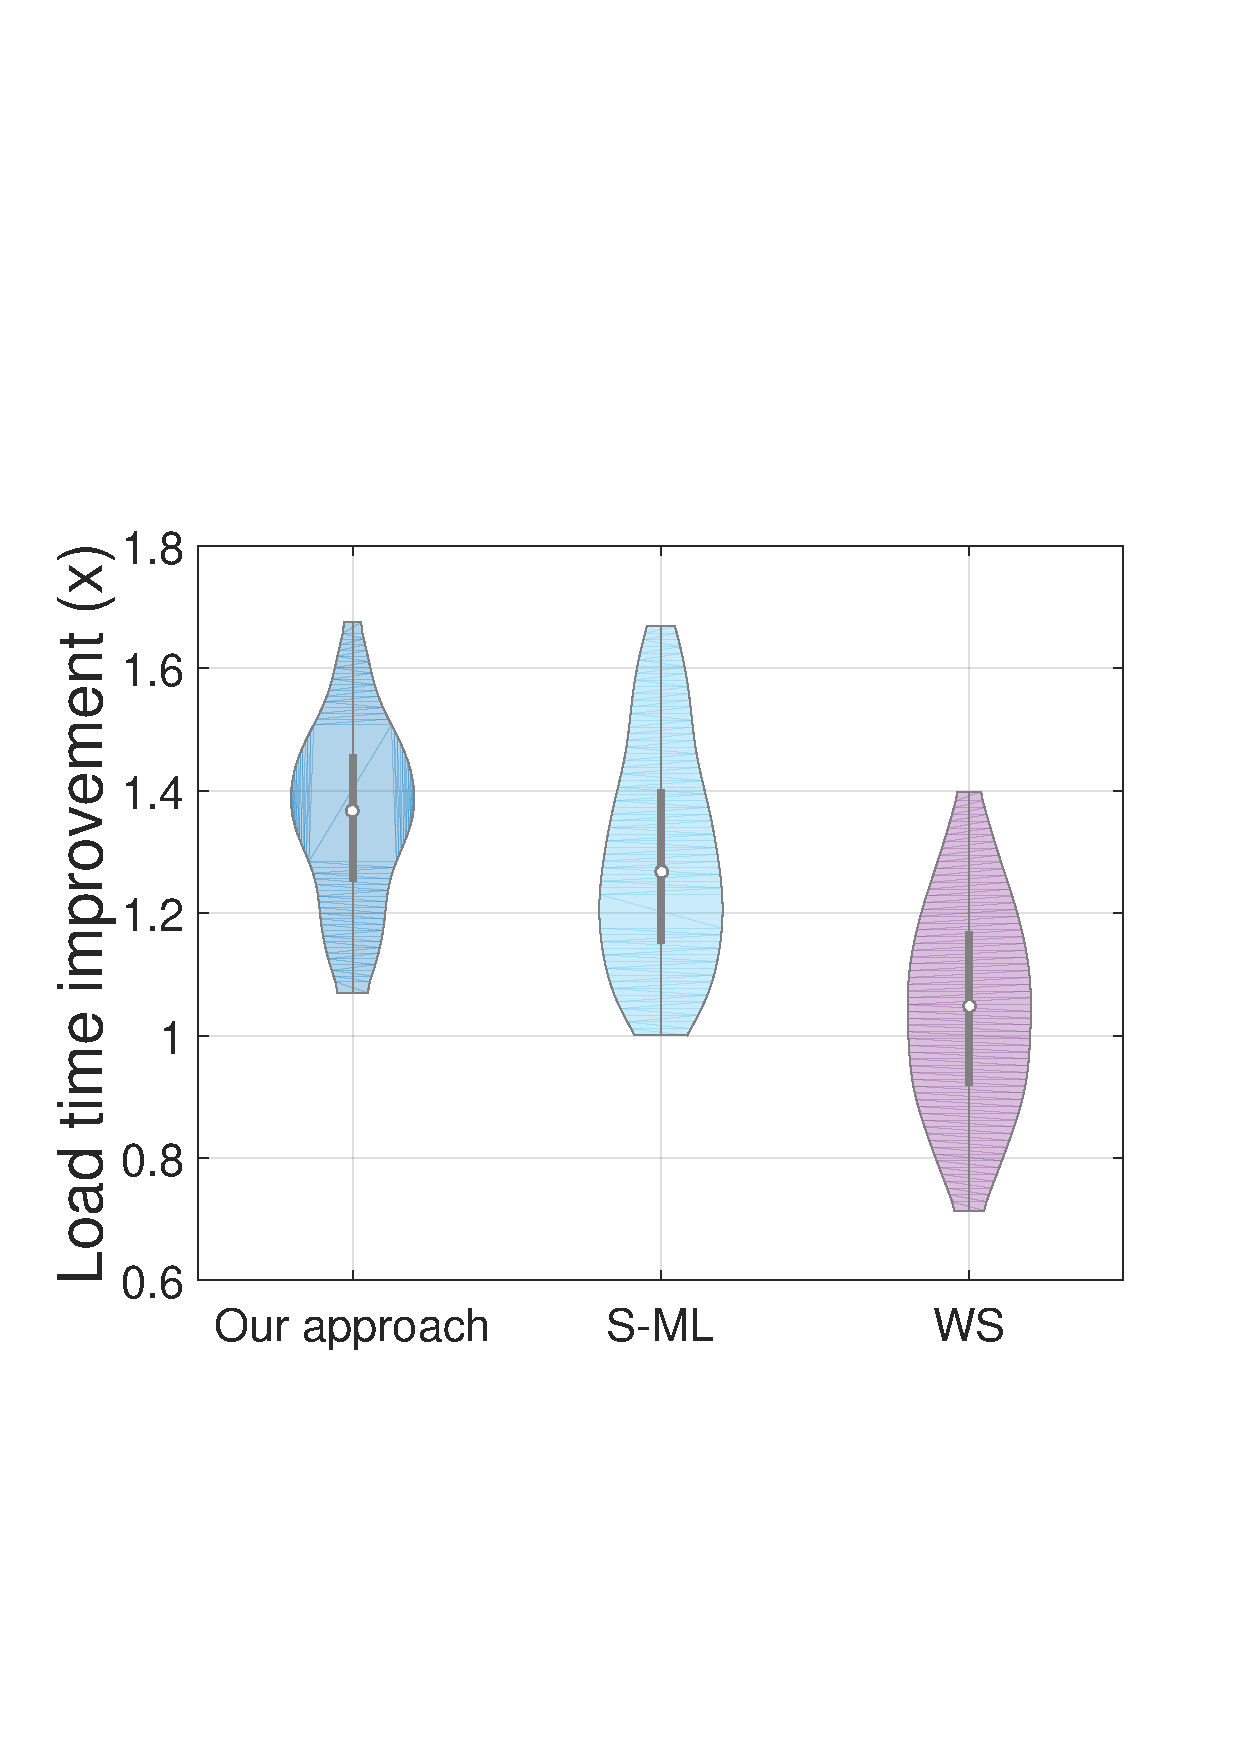
\includegraphics[width=0.24\textwidth]{figure/loadtime.pdf}}
    \hfill
	\subfloat[Energy Consumption]
    {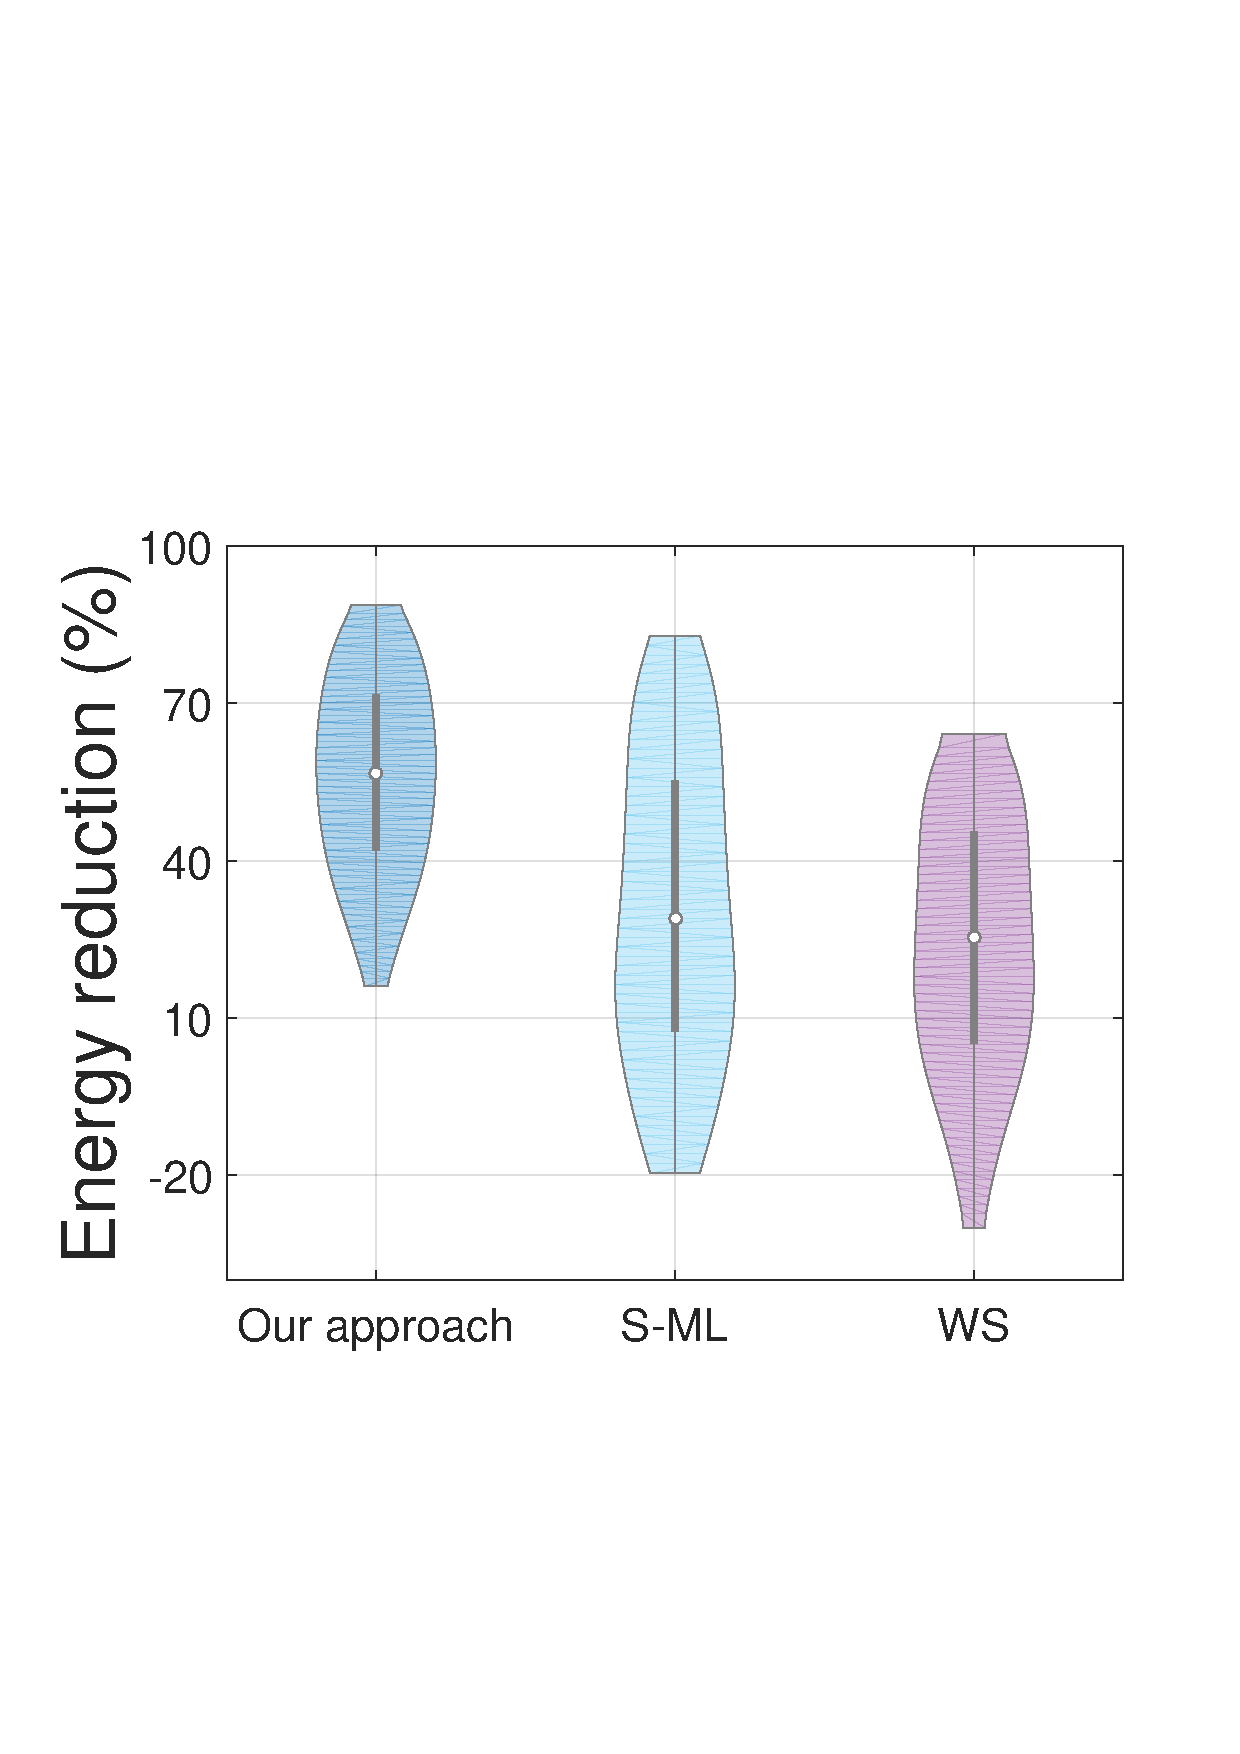
\includegraphics[width=0.241\textwidth]{figure/energy.pdf}}
    \hfill

    \caption{Violin plots showing the distribution for our approach, \SML and \WS in different network environments for three evaluation metrics: load time (a), energy reduction (b). The baseline is the best-performing Linux CPU governor. The thick line shows
where 50\% of the data lies. The white dot is the position of the median.}
    \label{fig:cpother}
    \vspace{-3mm}
\end{figure}


\section{Experimental Results\label{sec:experimental}}
%In this section, we first compare our approach against the best-performing Linux governor found from the five standard governors. We then
%evaluate our approach against two competitive web-aware schedulers, showing that our approach consistently outperforms
%the state-of-the-arts across all
%evaluation metrics. Finally, we analyze the working mechanism of our approach and compare it to the \oracle performance.

The violin plot in Figure~\ref{fig:cpother} compares our approach against two state-of-the-arts, \SML and \WS, across networking
environments and webpages. The baseline is the best-performing Linux CPU governor found for each webpage. The width of each violin
corresponds to the proportions of webpages with a certain improvement. The white dot denotes the median value, while the thick black line
shows where 50\% of the data lies.
The overhead of network monitoring,
extracting features, prediction and configuring frequency is
small. It is less than 7% of the turnaround time, which is
included in all our experimental results

On average, all approaches improve the baseline and the highest improvement is given by our approach. This confirms our hypothesis that
knowing the characteristics of the web content can improve scheduling decisions. If we look at the bottom of each violin, we see that \WS
and \SML can lead to poor performance in some cases. For example, \WS gives worse performance for 40\% of the webpages, with up to 30\%
slowdown for load time. \SML delivers better performance when compared with \WS, due to the more
advanced modeling technique that it employs. However, \SML also gives worse performance for 18\% and 17\% of the webpages for loadtime,
energy respectively, and can consume up to 20\% more energy than the baseline. The unstable performance of \WS and \SML is because they are
unaware of the network status, and thus lead to poor performance in certain environments. By contrast, our approach never gives worse
performance across networking environments and webpages. Finally, consider now the improvement distribution. There are more data points at
the top of the diagram under our scheme. This means our approach delivers faster load time and greater reduction on energy and \EDP when
compared with \WS and \SML. Overall, our approach outperforms the competitive approaches with an average improvement of 21\% and 39.2\% respectively for load time and energy, and without ever giving worse performance when compared with the baseline. We also
evaluate the performance of our techniques when web caching is enabled. The results show that our approach still outperforms the other two
methods with similar improvements.





%If we want to optimize for load time, there is no big difference between different network environments in Figure~\ref{fig:distribution}(a),
%we should always run the rendering process
%on the fast, big core (A15) with a frequency of at least 1.6 GHz. For this
%optimization goal, good network environments benefit from high performance A15 core with
%higher frequency(up to 1.9GHz) than poor network environments which prefer to run at a lower frequency (1.6 GHz to 1.8 GHz).
%The reasons that poor network conditions benefit from a lower frequency is because of CPU throttling~\cite{cputhrottling}, i.e. the hardware will automatically
%drop the frequency if the CPU becomes too hot when operating at a higher
%frequency for a while. We also found that running the rendering process at 2.0 GHz (a
%default setting used by most Linux performance governor) does not lead to
%better load time because of frequent CPU throttlings.
%
%When optimizing for energy consumption, most websites prefer to be scheduled on the energy-efficient core A7 or A15 with low frequency.
%As we can see from Figure~\ref{fig:distribution}(b), for regular 2G network, all of websites are scheduled on the A7 core with low frequency because of the adverse
%network condition, and around 46\% of the simple websites benefit from the
%A7 core with 0.4GHz. Furthermore, when the network conditions get improved, more websites can get benefit
%from A15 core. Supposing the user is under WiFi network environment, both $browser$ and $render$
%are more possible be scheduled on the big core with higher frequency, for instance, and around 47\% websites chose A15(1.2GHz) to render
%their websites.
%For EDP in Figure~\ref{fig:distribution}(c), using the A7 core benefits some websites but the ideal processor operating
%frequency leans towards a median value of the available frequency range. This
%is not supervising as EDP is a metric to quantify the trade-off between load
%time and energy consumption.


%\subsubsection{Prediction accuracy}



%Our approach gives correct predictions for 82.9\%, 88\% and 85\% of the webpages for load time, energy consumption and \EDP respectively.
%For those webpages that our approach does not give the best configuration, the resultant performance is not far from the optimal.

%Figure~\ref{fig:oracle} compares our approach with the \oracle predictor. The \oracle predictor named after its ability to make prophetic
%predictions, is able to predict the best possible configuration. This comparison indicates how close our approach is to the theoretically
%perfect solution. As can be seen from the diagram, our approach achieves 82\%, 92\% and 90\% of the \oracle performance for load time,
%energy consumption, and \EDP respectively. Although building a prefect predictor is almost impossible in reality, but the prediction accuracy can be improved through using more training %examples. Overall, the performance of our approach is not far from the performance given by an \oracle predictor.


